\section{图的着色}
\subsection{边着色}

\begin{definition}
设$G$是图,对$G$的边进行染色,若\textcolor{red}{相邻边染不同
颜色},则称\textcolor{red}{对$G$进行正常边着色}. 如果能用$k$种颜色对图$G$进行正常边着色,称$G$是\textcolor{red}{$k$边
可着色}的. 对$G$进行正常边着色需要的最少颜色
数,称为$G$的\colorbox{yellow}{\textcolor{red}{边色数}},记为:\colorbox{yellow}{$\chi^{\prime}(G)$}.
\begin{note}
	\colorbox{yellow}{$\chi^{\prime}(G)\geq \varDelta(G)$}
\end{note}
\end{definition}

\subsubsection{偶图的边色数}
\begin{theorem}
	\colorbox{yellow}{$\chi^{\prime}(K_{m,n})= \varDelta$}.
\end{theorem}

\begin{theorem}[哥尼,1916]
	若G是偶图,则 
	\colorbox{yellow}{$\chi^{\prime}(G)= \varDelta$}.
\end{theorem}

\subsubsection{简单图的边色数}

\begin{lemma}
设$G$是简单图,$x$与$y_1$是$G$中不相邻的两个顶点,$\pi$
是$G$的一个正常$k$边着色. 若对该着色$\pi$,$x$,$y_1$以及与$x$相邻
点均至少缺少一种颜色,则$G+xy_1$是$k$边可着色的.
\end{lemma}
\begin{figure}[H]
	\small
	\centering 
	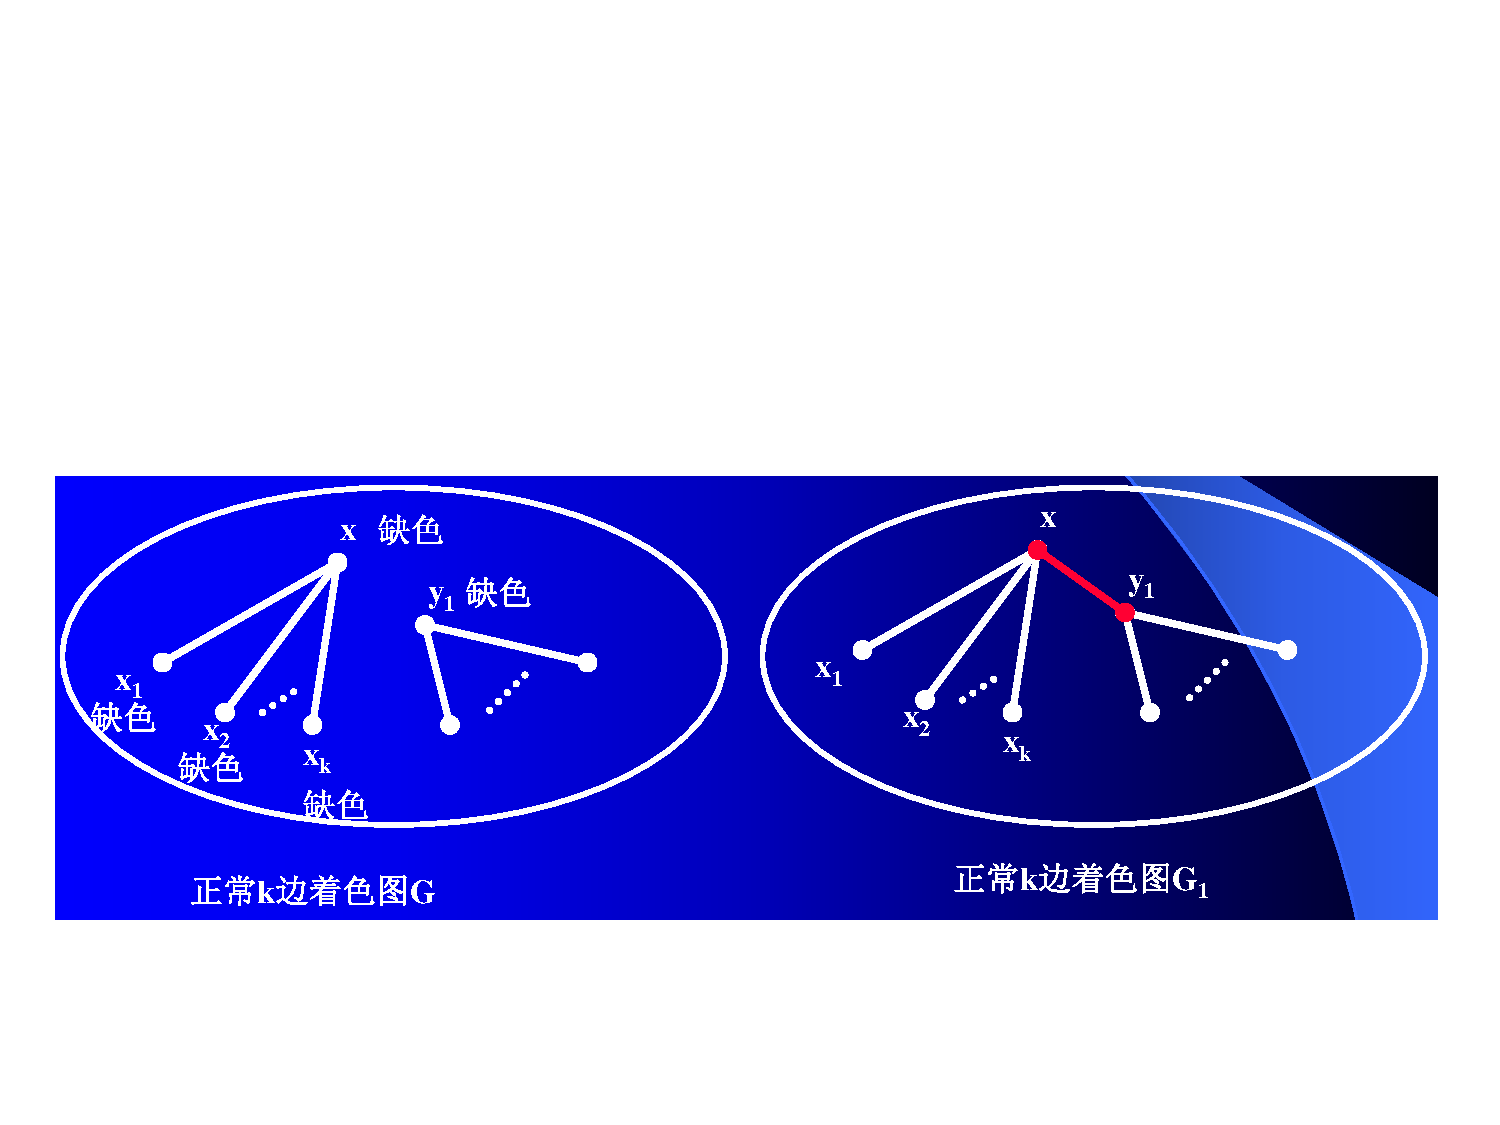
\includegraphics[scale=0.6]{image/CH7_bianzhuose.pdf}  
	%\caption{信息包结构} 
	\label{figkk1ik}  
\end{figure}
\begin{note}
\textcolor{red}{若点$u$关联的边的着色没有用到色$i$,则称点$u$缺$i$色}.
\end{note}
\begin{theorem}[维津定理,1964]
	若G是简单图,则 
	\[
	\colorbox{yellow}{$\chi^{\prime}(G)= \varDelta$} \mbox{or}\colorbox{yellow}{$ \chi^{\prime}(G)= \varDelta+1$}.
	\]
\end{theorem}
\begin{corollary}
	\begin{enumerate}
		\item $G$为简单图. 若$G$中只有一个最大度点
		或恰有两个相邻的最大度点,则:
		\[
		\colorbox{yellow}{$\chi^{\prime}(G)= \varDelta$}.
		\]
		\item $G$为简单图. 若点数$n=2k+1$且边数$m>k\varDelta$,则:\colorbox{yellow}{$\chi^{\prime}(G)= \varDelta+1$}.
		\begin{note}
			在应用题中求边色数,该结论很常用
		\end{note}
		\item 设$G$是奇数阶$\varDelta$正则简单图,若$\varDelta>0$,则:\colorbox{yellow}{$\chi^{\prime}(G)= \varDelta+1$}.
\end{enumerate}
\end{corollary}
\begin{note}
	\begin{enumerate}
		\item n方体的边色数为 \uline{n}.
		\item 彼得森图的边色数为 \uline{4}.
		\item $n$ 为奇数,$\chi^{\prime} (K_n) = (n - 1) + 1 = n,\chi^{\prime}  (C_n) = 2 + 1 = 3$.
		\item $n$ 为偶数,$\chi^{\prime} (K_n) = n - 1 ,\chi^{\prime}  (C_n) = 2$.
	\end{enumerate}
\end{note}
	
\subsection{点着色}
\begin{definition}
	设$G$是图,对$G$的顶点进行染色,若\textcolor{red}{使得相邻
		顶点着不同颜色},则称\textcolor{red}{对$G$进行正常顶点着色}. 如果能用$k$种颜色对图$G$进行正常顶点着色,称$G$是\colorbox{yellow}{\textcolor{red}{$k$(顶点)
			可着色}}的. 对$G$进行正常顶点着色需要的最少颜色
	数,称为$G$的\colorbox{yellow}{\textcolor{red}{(点)色数}},记为:\colorbox{yellow}{$\chi(G)$}.
\end{definition}
	\begin{note}
	\textcolor{red}{色数为$k$的图称为$k$色图}.
\end{note}
\begin{theorem}[维津定理,1964]
	\label{jjjgtbbb}
	对$\forall \quad G$,有:\colorbox{yellow}{$\chi(G)\leq \varDelta+1$}.
\end{theorem}

\noindent \textcolor{ecolor}{\bfseries 着色算法}\quad 设$G=(V, E), V= \{v_1,v_2,\cdots,v_n\}$,色集合$C=\{1,2,\cdots,\varDelta+1\}$,
着色方案为$\pi$.
\begin{enumerate}
	\item 令$\pi(v_1)=1, i=1$;
	
	\item \label{gggg}若$i=n$,则停止;否则令:
	\[
	\colorbox{yellow}{$C(v_{i+1})=\{\pi(v_j)|j\leq i \mbox{并且}v_j\mbox{与}v_{i+1} \mbox{相邻} \}   $}
	\]
	设$k$是$C-C(v_{i+1})$中最小整数,令\colorbox{yellow}{$ \pi(v_{i+1})=k  $};
.	\item 令$i=i+1$,转\ref{gggg}.
\end{enumerate}

\begin{example}
	给出下图的$\varDelta+1$正常点着色.
\begin{figure}[htbp]
	\centering
	\begin{minipage}{0.49\linewidth}
		\flushright
		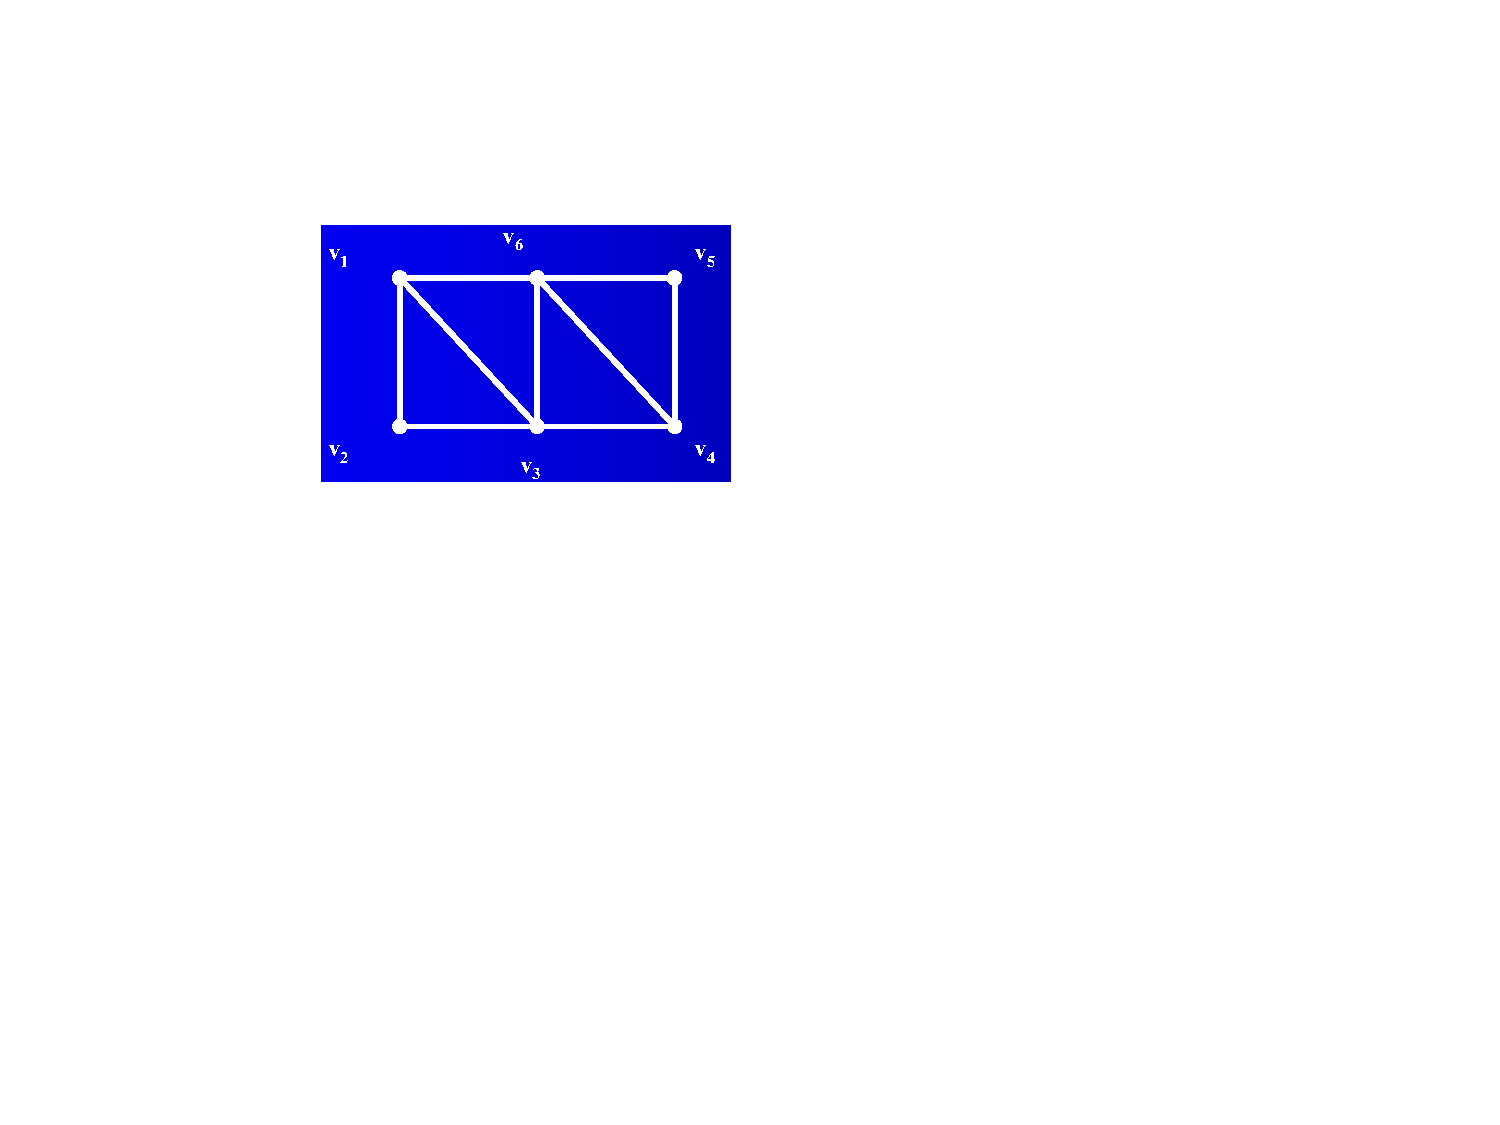
\includegraphics[scale=0.635]{image/CH7_dianzhuose1.pdf}  
		%\caption{chutian1}
		\label{chutian1}%文中引用该图片代号
	\end{minipage}
	%\qquad
	\begin{minipage}{0.49\linewidth}
		\centering
	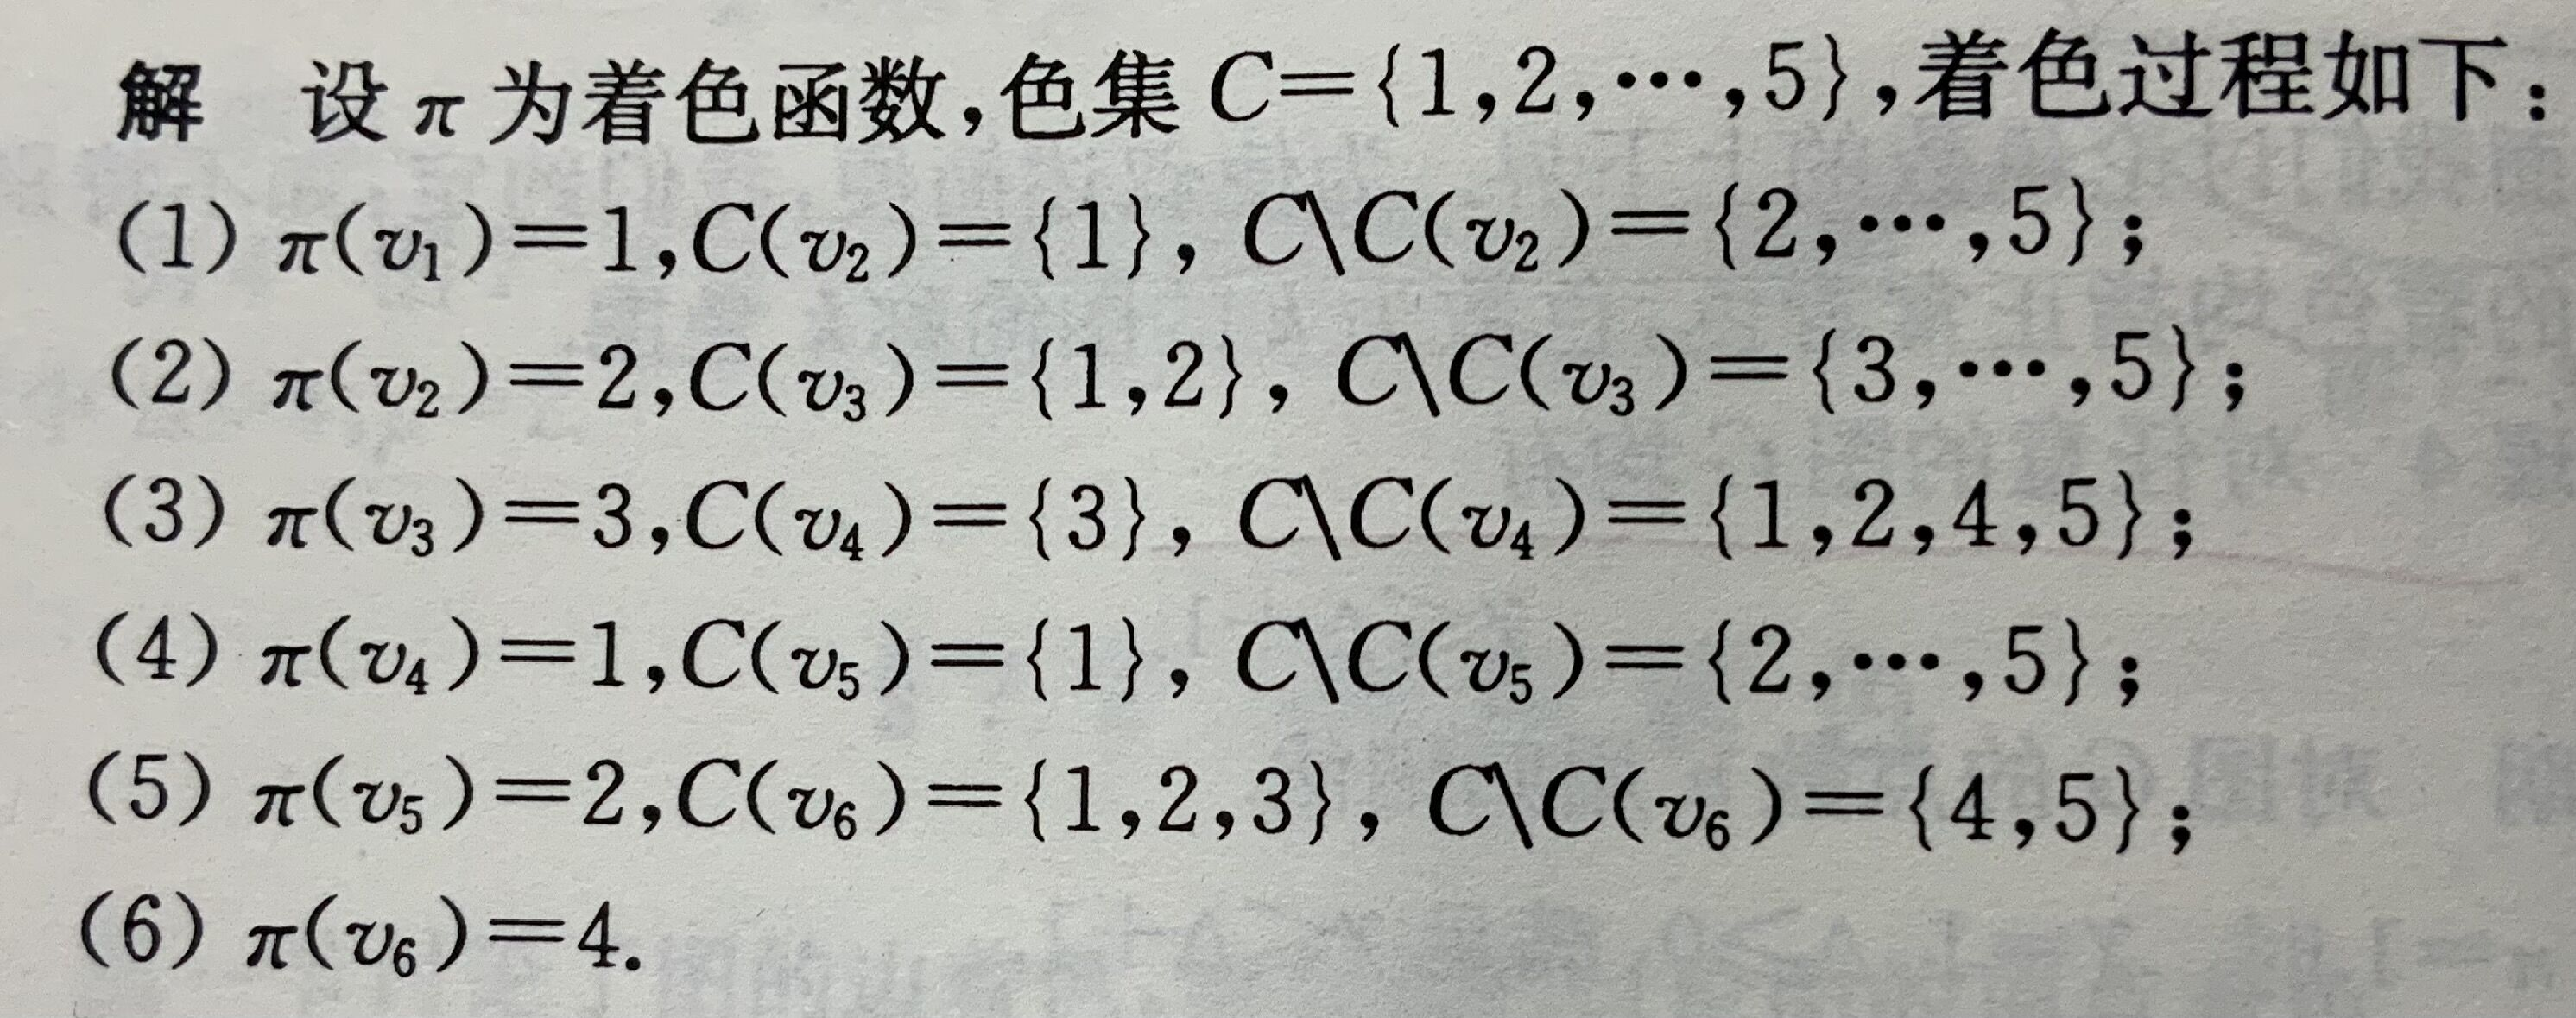
\includegraphics[width=0.9\linewidth]{image/CH7_dianzhuose.pdf} 
		%\caption{chutian2}
		\label{chutian2}%文中引用该图片代号
	\end{minipage}
\end{figure}
\end{example}


\begin{note}
	着色算法能保证最多使用$\varDelta+1$中颜色给一个图正常着色,但不能保证使用颜色数一定是最少的.Welsh—Powell稍微对上面算法做了一个修改,着色时
	按最大度优先策略.
\end{note}

\begin{theorem}[布鲁克斯,1941]
	若G是连通的单图,并且它
	既不是奇圈,又不是完全图, 则:\colorbox{yellow}{$\chi(G)\leq \varDelta$}.
\end{theorem}



\begin{definition}
	 设 $G$ 是至少有一条边的简单图, 定义:
\[
\Delta_{2}(G)=\max _{u \in V(G)} \max _{\substack{v \in N(u) \\ d(v) \leq d(u)}} d(v)
\]
其中 \( N(u) \) 为 \( G \) 中点 \( u \) 的邻域. 称 \( \Delta_{2}(G) \) 为 \( G \) 的\textcolor{red}{次大度}.
如果令:
\[
\colorbox{yellow}{$V_{2}(G)=\{v \mid v \in V(G), N(v) \text { 中存在点 } u, \text { 满足 } d(u) \geq d(v)\}$}
\]
那么,
\[
\colorbox{yellow}{$\Delta_{2}(G)=\max \left\{d(v) \mid v \in V_{2}(G)\right\}$}
\]
\end{definition}

\begin{theorem}
	\label{jjjhhlll}
	设G是非空简单图,则:\colorbox{yellow}{$\chi(G)\leq \varDelta_2(G)+1$}.
\end{theorem}
\begin{note}
	定理\ref{jjjhhlll}是对定理\ref{jjjgtbbb}改进.
\end{note}

\begin{corollary}
	设$G$是非空简单图,若$G$中最大度点互不邻接,
	则:\colorbox{yellow}{$\chi(G)\leq \varDelta(G)$}.
\end{corollary}


\begin{theorem}[希伍德]
对任意平面图,均有$\chi \leq 5$.
\end{theorem}
\begin{note}
	\begin{enumerate}
	\item n方体的点色数为 \uline{2}.
		\item 彼得森图的点色数为 \uline{3}.
	\end{enumerate}
\end{note}

\subsection{色多项式}

由点色数 \( \chi(G) \) 和色多项式 \( {P}_{{k}}(\mathrm{G}) \) 的定义可得:
\begin{enumerate}
	\item 若 \( k<\chi(G) \), 则 \( {P}_{{k}}({G})={0} ; \chi(G)=\min \left\{k \mid P_{k}(G) \geq 1\right\} \).
	\begin{note}
		通过色多项式方法求色数原理.
	\end{note}
	\item 若 \( G \) 为空图, 则 \( P_{k}(G)=k^{n} \) .
	\item \colorbox{yellow}{$ P_{k}\left(K_{n}\right)=k(k-1) \ldots(k-n+1) $}.
\end{enumerate}



\noindent {\bfseries \textcolor{ecolor}{色多项式的两种求法}}
\subsubsection{递推计数法}
\begin{theorem}
	设$G$为简单图,则对任意,有
	\begin{equation*}
		\colorbox{yellow}{$
		\begin{split}
			&P_k(G)=P_k(G-e) - P_k(G\cdot e)\quad \mbox{减边, $G$的边数较少时}\\
			&P_k(G-e)=P_k(G)+ P_k(G\cdot e)\quad \mbox{加边, $G$的边数较多时}\\
		\end{split}
	$}
	\end{equation*}
\end{theorem}
\begin{corollary}
设$G$是单图,$e=uv$是$G$的一条边,且$d(u)=1$,则:$P_k(G)=(k-1)P_k(G-u) $.
\end{corollary}

\subsubsection{理想子图计数法(必考)}

\begin{definition}
设$H$是图$G$的生成子图. 若$H$的每个分支均为
完全图,则称$H$是$G$的一个\colorbox{yellow}{\textcolor{red}{理想子图}}. 用\colorbox{yellow}{$N_r(G)$}表示$G$的具有\colorbox{yellow}{ $r$ }个分支的理想子图的个数($r\geq \omega(G)$).
\end{definition}

对于$n$阶简单图,有理想子图法色多项式计数公式:
\[\colorbox{yellow}{$P_k(G)=\sum\limits_{i=1}^{n} N_i(\overline{G})\left[k\right]_i \quad \left[k\right]_i = k(k-1)(k-2)\cdots (k-i+1)$}
\]
\begin{note}
	\begin{enumerate}
	\item $N_n(G)=1$.
	\item $N_{n-1}(G)=m$.
	\item 若$k<\omega(G)$,则$N_k(G)=0$.
\end{enumerate}	
\end{note}

$\overline{G}$的伴随多项式:
\[\colorbox{yellow}{$h(\overline{G},x)=\sum\limits_{i=1}^{n} r_ix^i \quad r_i= N_i(\overline{G}),x^i=\left[k\right]_i$}
\]

\begin{theorem}
	若$G$有$t$个分支$H_1,H_2,\cdots,H_t$,且$H_i$的伴随多项式为$h(H_i, x), 
	i=1,2,…,t$, 则:
	\[
	\colorbox{yellow}{$h(G, x)=\prod\limits_{i=1}^{t} h\left(H_{i}, x\right)$}
	\]
\end{theorem}

\noindent \textcolor{red}{图$G$色多项式求解步骤:}
\begin{enumerate}
	\item 画出$G$的补图$\overline{G}$;
	\item 求出$\overline{G}$中个分支的伴随多项式;
	\item 求出$\overline{G}$的伴随多项式;
	\item 求出$G$的色多项式.
\end{enumerate}












